%!TEX ROOT=formularioFisica.tex

\section{Appendice}
\subsection{Proporzionalit�}
Per esprimere la proporzionalit� si utilizza il simbolo $\propto$.\\
Si dicono \textbf{direttamente proporzionali} due variabili $x,y$ se
\begin{equation*}
y = kx\,(y\propto x)
\end{equation*}
Ovvero se all'aumentare di $x$ aumenta anche $y$.\\ [\baselineskip]
Si dicono \textbf{inversamente proporzionali} due variabili $x,y$ se 
\begin{equation*}
xy = k\,\left(y\propto\frac{1}{x}\right)
\end{equation*}
  
\subsection{Distanza}

La distanza tra due punti � un concetto fondamentale e si calcola 
\begin{equation*}
d=\sqrt{(x2-x1)^{2}+(y2-y1)^{2}}
\end{equation*}
\begin{center}     
	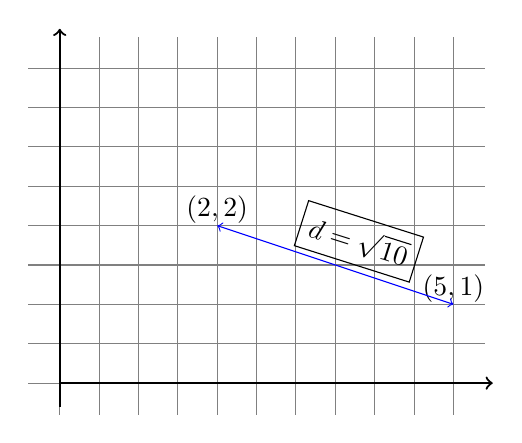
\begin{tikzpicture}
		\draw[step=0.5cm,gray](-0.9,-0.9) grid (4.9,3.9) ;
		\draw[thick,->,black] (-.5,-0.8) -- (-0.5,4) ;
		\draw[thick,->,black]  (-.5,-0.5)--(5,-0.5);
		\node at (1.5,1.7) {$(2,2)$};
		\node at (4.5,0.7){$(5,1)$};
		\draw[<->,blue](1.5,1.5)--(4.5,0.5);
		
		\node[draw,rotate=-17.6] at (3.3,1.3){$d=\sqrt{10}$};	
\end{tikzpicture}            
\end{center}

\subsection{Notazione scientifica}
I valori ottenuti in fisica possono presentare a volte molti zeri, per ovviare alla difficolt� di 
lettura di questi numeri si utilizza la notazione scientifica che consiste nello scrivere qualunque
numero come 
\begin{equation*}
\text{Numero}=x\cdot 10^{y}
\end{equation*}
con x tra 0 e 10 e con untima cifra diversa da 0\\
Dunque $107,000=1,07\cdot10^{5}$ e $0.0000098=9,8\cdot10^{-8}$ 
Frequentemente $10^{y}$ viene ancora semplificato con alcuni prefissi:

\begin{center}
   \begin{tabular}{c c c}
     & Prefisso & Nome prefisso\\ \hline
     $10^{18}$ & E &  esa\\ \hline
     $10^{15}$ & P & peta\\ \hline
     $10^{12}$ & T & tera\\ \hline
     $10^{9}$ & G & giga\\ \hline
     $10^{6}$ & M & mega\\ \hline
     $10^{3}$ & k & kilo\\ \hline
     $10^{2}$ & h & etto\\ \hline
     $10^{-1}$ & d & deci\\ \hline
     $10^{-2}$ & c & centi\\ \hline
     $10^{-3}$ & m & milli\\ \hline
     $10^{-6}$ & $\mu$ & micro\\ \hline
     $10^{-9}$ & n & nano\\ \hline
     $10^{-12}$ & p & pico\\ \hline
     $10^{-15}$ & f & femto\\ \hline
     $10^{-18}$ & a & atto\\
  \end{tabular}
\end{center}

\subsection{Quadrato}
Il quadrato � una figura regolare con 4 lati.\\ Definendo $l=$lunghezza del lato si calcola
\begin{equation*}
\text{Area}=l^{2}\quad\text{Diagonale}=l\sqrt{2}
\end{equation*}
\begin{center}     
	\begin{tikzpicture}
		\draw (0,0) -- (2,0) -- (2,2) -- (0,2) -- cycle;
		
		\node at (1,0.1) {$l$};
	\end{tikzpicture} 
\end{center}

\subsection{Triangolo}
Il triangolo � una figura con tre lati. Esistono svariati tipi di traingoli ma quelli piu comuni in 
fisica sono i trangoli rettangoli (ovvero quei triangoli che hanno un angolo di $90$ gradi).

\begin{center}     
	\begin{tikzpicture}
		\draw (0,0) -- (4,0);
		\node at (-0.15,-0.1) {C};
		\node at (2,1.1) {c};
		\draw (4,0) -- (0,2);
		\node at (4.2,-0.1) {A};
		\node at (-0.2,1) {a};
		\node at (3.5,0.1) {$\alpha$}; 
		\draw (0,2) -- (0,0);
		\node at (0,2.15) {B};
		\node at (0.175,1.7) {$\beta$};
		\node at (2,-0.2){b};
	\end{tikzpicture}
\end{center}
Si definisce $c$ (il lato pi� lungo) ipotenusa, $b$ (lato di media lunghezza) cateto maggiore e
$a$ (lato pi� corto)\\
Alla base di tutte le formule sul triangolo rettangolo sta il Teorema di Pitagora:
\begin{equation*}
c^2=a^2+b^2
\end{equation*}
Oltre a questa formula sono fondamentali anche:
\begin{align*}
	b&=c\cos\alpha\quad\text{e}\quad a=c\sin\alpha\\
	a&=c\cos\beta\quad\text{e}\quad b=c\sin\beta
\end{align*}
Al seno e al coseno va aggiunta la tangente che si definisce:
\begin{equation*}
\tan x = \frac{\sin x}{\cos x}
\end{equation*}
Attraverso la tangente:
\begin{equation*}
a=b\tan\alpha \qquad
b=a \tan\beta
\end{equation*}  
Un altra formula importante �
\vspace{-0.5cm}
\begin{center}
\begin{equation*}
\cos{x}^{2}+\sin{x}^{2}=1 
\end{equation*}
\end{center}
che si usa per ottenere il il seno quando si ha il coseno e viceversa.
\subsection{Cerchio}

Il cerchio � una figura fondamentale, si dimostra che: 
\begin{align*}
\text{Circonferenza}&=2\pi r\\
\text{Area}&=\pi r^2
\end{align*}

\begin{center}     
	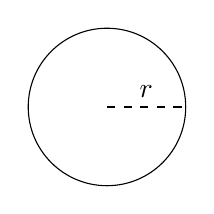
\begin{tikzpicture}
	\draw (0,0) circle (1cm);
	\draw [dashed](0,0)--(1,0);
	\node at (0.5,0.2) {$r$};
	\end{tikzpicture}
\end{center}
$\pi$ � un numero irrazionale definito appunto come rapporto la lunghezza della circonferenza e il 
diametro, il suo valore approssimato � $3,14159$. \\	
Facendo ruotare un cerchio di $180$ gradi si ottiene una sfera. Il volume di una sfera � pari a
\begin{equation*}
V=\frac{4}{3}\pi r^{2}
\end{equation*}

\subsection{Equazioni}
Esistono svariati tipi di equazioni, tra le pi� comuni vi sono quelle di secondo grado. Per risolvere le equazioni   $ax^{2}+bx+c=0$  
si usa la seguente formula:

\begin{equation*}
x_{1/2}={\frac{-b\pm\sqrt{b^{2}-4ac}}{2a}}
\end{equation*}
Per risolvere sistemi di equazioni come questo
\begin{equation*}
\begin{cases}  ax+by= \textcolor{red}{c}, \\ dx+ey= \textcolor{red}{f},\\ 
\end{cases}
\end{equation*}
 si pu� usare il teorema di Cramer:

\begin{equation*}
  x=\dfrac{\begin{vmatrix}[1]
  \textcolor{red}{c} & b \\  
  \textcolor{red}{f} & e 
\end{vmatrix}}{\begin{vmatrix}[1] 
  a & b \\ d & e \end{vmatrix}}= 
\dfrac{\textcolor{red}{c}e-b\textcolor{red}{f}}{ae-bd}     \quad 
 y=\dfrac{\begin{vmatrix}[1]  a &\textcolor{red}{c} \\ d &  \textcolor{red}{f} \end{vmatrix}}
 {\begin{vmatrix}[1]  a & b \\ d & e \end{vmatrix}}= 
\dfrac{a \textcolor{red}{f}- \textcolor{red}{c}d}{ae-bd}
\end{equation*}
Con questa logica si possono risolvere sistemi con anche pi� equazioni.

%!TEX ROOT=formularioFisica.tex

\section{Vettori}
Questa prima sezione � introduttiva ad uno dei concetti pi� comuni in fisica: il \emph{vettore}.\\
Un vettore pu� essere rappresentato in molti modi, tra cui:
\begin{equation*}
\vec{v} = 
\begin{bmatrix}[1]
a\\b\\\vdots
\end{bmatrix} = 
(a, b, \dots)
\end{equation*}
Un vettore � composto di un numero definito di \emph{componenti}, solitamente una per ciascuna
dimensione in cui si lavora. Quindi � decisamente pi� comune trovare vettori \emph{bidimensionali}
che non con un numero maggiore di componenti.\\
\begin{center}
	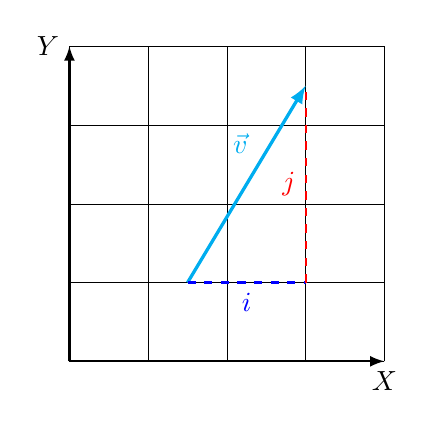
\begin{tikzpicture}
		\draw[step=1, very thin] (0,0) grid (4,4);
		\draw[-latex, thick] (0,0) -- (4,0)
			node[pos=1, below]{$X$};
		\draw[-latex, thick] (0,0) -- (0,4)
			node[pos=1, left]{$Y$};
		\draw[-latex, very thick, cyan] (1.5, 1) -- (3, 3.5)
			node[pos=0.6, above left]{$\vec{v}$};
		\draw[dashed, thick, blue] (1.5, 1) -- (3, 1)
			node[pos=0.5, below]{$i$};
		\draw[dashed, thick, red] (3, 1) -- (3, 3.5)
			node[pos=0.5, left]{$j$};
	\end{tikzpicture}
\end{center}
In questa immagine � possibile vedere un vettore $\mathcolor{cyan}{\vec{v}}(\mathcolor{blue}{i},
\mathcolor{red}{j})$ e le sue componenti.\\[\baselineskip]
D'ora in poi sar� dato per scontato che i vettori siano bi-dimensionali.

\subsection{Operazioni tra vettori}
Le operazioni come addizione e sottrazione funzionano molto semplicemente sommando algebricamente
le componenti tra di loro:
\begin{equation*}
\mathcolor{red}{\vec{v_1}\left(a_1, b_1\right)} \pm 
\mathcolor{blue}{\vec{v_2}\left(a_2, b_2\right)} = 
\mathcolor{purple}{\vec{v}}\left(\mathcolor{red}{a_1}\pm \mathcolor{blue}{a_2}, 
\mathcolor{red}{b_1}\pm \mathcolor{blue}{b_2}\right)
\end{equation*}

La moltiplicazione tra vettori pu� avere come risultato o un \emph{vettore} o uno \emph{scalare}.

\subsubsection{Prodotto scalare}
\begin{equation*}
\mathcolor{red}{\vec{v_1}} \cdot \mathcolor{blue}{\vec{v_2}} = 
\mathcolor{red}{a_1}\mathcolor{blue}{a_2} + \mathcolor{red}{b_1}\mathcolor{blue}{b_2}
\end{equation*}
Come si pu� notare il prodotto scalare tra due vettori torna uno scalare (ovvero un numero).
In fisica per� � molto pi� comune trovare questa definizione di prodotto scalare:
\begin{equation*}
\mathcolor{red}{\vec{v_1}} \cdot \mathcolor{blue}{\vec{v_2}} =
\norm{\mathcolor{red}{\vec{v_1}}}\cdot\norm{\mathcolor{blue}{\vec{v_2}}}\cos\theta
\end{equation*}
$\norm{\vec{v}}$ � il modulo del vettore $\vec{v}$, ovvero la sua lunghezza. $\theta$ � l'angolo
formato dai due vettori.

\subsubsection{Prodotto vettoriale}\label{subsec:vettori:prodottoVettoriale}
\begin{equation*}
\mathcolor{red}{\vec{v_1}} \times \mathcolor{blue}{\vec{v_2}} =
n\norm{\mathcolor{red}{\vec{v_1}}}\cdot\norm{\mathcolor{blue}{\vec{v_2}}}\sin\theta
\end{equation*}
$\norm{\vec{v}}$ � il modulo del vettore $\vec{v}$, ovvero la sua lunghezza. $\theta$ � l'angolo
formato dai due vettori. $n$ � la \emph{normale} del piano su cui stanno i vettori. Una \emph{normale}
� un vettore perpendicolare ad un oggetto dato.\\
Per scoprire la direzione del nuovo vettore si pu� usare la cos� detta 'regola della mano`. Essa dice:
\begin{enumerate}
	\item Usare il pollice della mano destra in direzione e verso del \textbf{primo} vettore
	\item Usare l'indice o le altre dite in direzione e verso del \textbf{secondo} vettore
	\item Il nuovo vettore avr� la direzione che attraversa il palmo perpendicolarmente e il verso 
	uscente dalla mano.
\end{enumerate}
